%
% File acl2021.tex
%
%% Based on the style files for EMNLP 2020, which were
%% Based on the style files for ACL 2020, which were
%% Based on the style files for ACL 2018, NAACL 2018/19, which were
%% Based on the style files for ACL-2015, with some improvements
%%  taken from the NAACL-2016 style
%% Based on the style files for ACL-2014, which were, in turn,
%% based on ACL-2013, ACL-2012, ACL-2011, ACL-2010, ACL-IJCNLP-2009,
%% EACL-2009, IJCNLP-2008...
%% Based on the style files for EACL 2006 by 
%%e.agirre@ehu.es or Sergi.Balari@uab.es
%% and that of ACL 08 by Joakim Nivre and Noah Smith

\documentclass[11pt,a4paper]{article}
\usepackage[hyperref]{acl2021}
\usepackage{times}
\usepackage{latexsym}
\usepackage{titlesec}
\usepackage{amsmath}
\usepackage{color,soul}
\setcounter{secnumdepth}{5}
\renewcommand{\UrlFont}{\ttfamily\small}
\usepackage{graphicx}
\graphicspath{{./images/}}
%\usepackage[parfill]{parskip}
\usepackage{booktabs}
\usepackage{array}

% This is not strictly necessary, and may be commented out,
% but it will improve the layout of the manuscript,
% and will typically save some space.
\usepackage{microtype}

\aclfinalcopy % Uncomment this line for the final submission
%\def\aclpaperid{***} %  Enter the acl Paper ID here

%\setlength\titlebox{5cm}
% You can expand the titlebox if you need extra space
% to show all the authors. Please do not make the titlebox
% smaller than 5cm (the original size); we will check this
% in the camera-ready version and ask you to change it back.

\newcommand\BibTeX{B\textsc{ib}\TeX}

\makeatletter
\renewcommand\paragraph{%
    \@startsection{paragraph}{4}{0mm}%
        {-\baselineskip}%
        {.5\baselineskip}%
        {\normalfont\normalsize\bfseries}}
\makeatother

\title{BigGreen at SemEval-2021 Task 1: \\
Lexical Complexity Prediction with Assembly Models}

\author{
  \textbf{Aadil Islam}\normalfont{,} \textbf{Weicheng Ma}\normalfont{, and} \textbf{Soroush Vosoughi}\\
  Department of Computer Science\\
  Dartmouth College\\
  \texttt{\{aadil.islam.21, weicheng.ma.gr, soroush.vosoughi\}@dartmouth.edu}
}

\date{}

\begin{document}
\maketitle

\begin{abstract}
  This paper describes systems submitted by team BigGreen to LCP 2021. We assemble a feature engineering-based model with a deep neural network model founded on BERT. The latter model contextualizes a target expression, given its sentence. While BERT is a strong model overall, the feature engineering-based model helps in extreme cases, eg. separating instances of easy and neutral difficulty. Our handcrafted features comprise a breadth of lexical, semantic, syntactic, and novel phonological measures. Additionally, visualizations of BERT attention maps offer insight into potential features that Transformers models may learn when fine-tuned for lexical complexity prediction. Our ensembled predictions score reasonably well for the single word subtask, and we demonstrate how it they can be harnessed to perform well on the multi word expression subtask too.
\end{abstract}

\section{Introduction}

Lexical simplification (LS) is the task of replacing difficult words in a text with simpler alternatives. It is applicable to reading comprehension, where early studies have shown infrequent words lead to more time spent by a reader fixated on it, and that ambiguity in a word's meaning adds to comprehension time \citep{raynerd86}. Complex word identification (CWI) is believed to be a fundamental step in the automation of lexical simplification \citep{shardlow2014open}. Early techniques for conducting CWI suffer from a lack of robustness, from simplifying all words to then study its efficacy \citep{devlintait}, to applying thresholds on features like word frequency \citep{10.1007/11573067_19}. 

This year's Lexical Complexity Prediction (LCP) shared task \citep{shardlow2020complex} forgoes the treatment of word difficulty as a binary classification task \citep{paetzoldspecia:2016:SemEval1, stajner-EtAl:2018:BEA} and instead measures degree of complexity on a continuous scale. This choice is intriguing as it mitigates a dilemma with previous approaches of having to treat words extremely close to a decision boundary (suppose a threshold deems a word's difficulty) identically to those that are far away, ie. extremely easy or difficult.

Teams are asked to submit predictions on unlabeled test sets for two subtasks: predicting on single word and multi word expressions (MWEs), respectively. For each subtask, \texttt{BigGreen} presents a machine learning-based approach that fuses the predictions of a feature engineering-based regressor with those of a feature learning-based deep neural network model founded on BERT \citep{DBLP:journals/corr/abs-1810-04805}. Our code is made available on GitHub.\footnote{\url{https://github.com/Aadil101/BigGreen-at-LCP-2021}}

\section{Related Work}

Previous studies have looked at estimating the readability of a given text at the sentence-level. \citet{10.2307/40011226} regresses the number of polysyllabic words in a given lesson against the mean score for students quizzed on said lesson, yielding the SMOG Readability Formula. \citet{10.2307/1473169} offer a list of 768 (later updated to 3,000) words familiar to grade-school students in reading, which they find correlates with passage difficulty. An issue with traditional readability metrics seems to be the loss of generality at the word-level.

Results from CWI at SemEval-2016 \citep{zampieriEtAl:2017:NLPTEA} suggest vote ensembling predictions of the best performing models as an effective strategy, while several top-performing models \citep{paetzoldspecia2016sv000gg, ronzanoetal2016taln, mukherjeeetal2016ju} appear to use linguistic information beyond word frequency. These findings inspires our use of ensemble techniques, and a foray into phonological features as a point of research. Results from CWI at SemEval-2018 show feature engineering-based models outperforming deep learning-based counterparts, despite the latter having generally better performances since SemEval-2016.

\section{Data}

\subsection{CompLex Dataset}

\begin{table}
  \centering
  \begin{tabular}{l|l|r|r|r}
    \toprule
    \centering
    Corpus & Subtask & Train &  Trial &  Test \\
    \midrule
    Bible & Single Word &   2574 &    143 &   283 \\
            & Multi Word &    505 &     29 &    66 \\
    \midrule
    Biomed & Single Word &   2576 &    135 &   289 \\
            & Multi Word &    514 &     33 &    53 \\
    \midrule
    Europarl & Single Word &   2512 &    143 &   345 \\
            & Multi Word &    498 &     37 &    65 \\
    \bottomrule
  \end{tabular}
  \caption{\label{tab:datasets} LCP train, trial, and test sets.}
\end{table}

\citet{shardlow2020complex} present CompLex, a novel dataset in which target expressions (single words or MWEs) are assigned continuous labels denoting their lexical complexity. Each label lies in range 0-1, a (normalized) average score given by employed crowd workers who record an expression's difficulty on a 5-point Likert scale. We define a sample's \textit{class} as the bin to which its complexity label belongs (bins corresponding to Likert points). Target expressions in CompLex have 0.395 average complexity and 0.115 standard deviation, reflecting an imbalance in favor of class 2 and 3 samples. 

Each target expression is accompanied by the sentence it was extracted from, drawn from one of three corpora (Bible, Biomed, and Europarl). A summary of the train, trial,\footnote{In our study we avoid the trial set as we find it to be less representative of the training data, opting instead for training set cross-validation, stratified by corpus and complexity label.} and test set samples is provided in Table \ref{tab:datasets}.

\subsection{External Datasets}

We use four additional corpora to extract term frequency-based features from:

\begin{itemize}
  \item \noindent \textbf{English Gigaword Fifth Edition} (Gigaword): this comprises articles from seven English newswires \citep{gigaword}.
  \item \noindent \textbf{Google Books Ngrams, version 2} (GBND): this is used to count occurences of phrases across a corpus of books, accessed via the PhraseFinder API \citep{phrasefinder}.
  \item \noindent \textbf{British National Corpus, version 3} (BNC): this is a collection of written and spoken English \citep{BNC}.
  \item \noindent \textbf{SUBTLEXus}: this consists of American English subtitles, offering a multitude of word frequency lists \citep{Brysbaert2009MovingBK}.
\end{itemize}

\section{BigGreen Systems \& Approaches}

In this section, we overview features fed to our feature engineering-based system, as well as training techniques for the feature learning-based model. Note that the fitted models for the single word subtask are then harnessed for the MWE subtask.

\subsection{Feature Engineering-based System}

\subsubsection{Feature Extraction}

We aim to capture a breadth of information pertaining to the target word and its context. Most features follow heavily right-skewed distributions, prompting us to consider logged and unlogged versions of features. For the MWE subtask, features are extracted independently for head and tail words.

\paragraph{Lexical Features}

These are features based on lexical information about the target word:

\begin{itemize}
  \item \textbf{Word length}: length of the target word.
  \item \textbf{Number of syllables}: number of syllables in the target word, via the Syllables library.\footnote{\url{https://github.com/prosegrinder/python-syllables}}
  \item \textbf{Is acronym}: whether the target word is a sequence of capital letters.
\end{itemize}
  
\paragraph{Semantic Features}

These features capture the target word's meaning:

\begin{itemize}
  \item \textbf{WordNet features}: the number of hyponyms and hypernyms associated with the target word in WordNet \citep{Fellbaum:2005}.
  \item \textbf{GloVe word embeddings}: we extract 300-dimension embeddings pre-trained on Wikipedia-2014 and Gigaword \citep{pennington2014glove} for each (lowercased) target word. 
  \item \textbf{ELMo word embeddings}: we extract for each target word a 1024-dimension contextualized embedding pre-trained on the One Billion Word Benchmark \citep{Peters:2018}.
  \item \textbf{GloVe context embeddings}: we obtain the average 300-dimension GloVe word embedding over each token in the given sentence.
  \item \textbf{InferSent context embeddings}: we obtain 4096-dimension InferSent embeddings \citep{conneau-EtAl:2017:EMNLP2017} for each sentence.
\end{itemize}

\paragraph{Phonetic Features}

These features compute the likelihood that consecutive soundable segments in the target word would arise in English language. We estimate ground truth transition probabilities between any two units (phonemes or characters) using Gigaword. 

\begin{itemize}
  \item \textbf{Phoneme transition probability}: we consider the min/max/mean/standard deviation over the set of transition probabilities for the target word's phoneme bigrams.
  \item \textbf{Character transition probability}: analogous to that above, over \textit{character} bigrams.
\end{itemize}

\paragraph{Word Frequency and N-gram}

These features are expressly included due to their expected importance, \citep{zampieriEtAl:2017:NLPTEA}. Gigaword is the main corpus from which we extract word frequency measures (for both lemmatized and unlemmatized target words), summed frequency of the target word's byte pair encodings (BPEs), and summed frequencies of bigrams and trigrams. We complement these features with IDF-based analogues. Lastly, we use the GBND, BNC, and SUBTLEXus corpora to extract secondary word frequency, bigram, and trigram measures. 

\paragraph{Syntactic Features}

These are features that assess the syntactic structure of the target word's context. We construct the constituency parse tree for each sentence using a Stanford CoreNLP pipeline \citep{manning-EtAl:2014:P14-5}.

\begin{itemize}
  \item \textbf{Part of speech (POS)}: tag is obtained using NLTK's \texttt{pos\_tag} \citep{Loper02nltk:the}.
  \item \textbf{Depth of parse tree}: the parse tree's height.
  \item \textbf{Depth of target word}: the distance between the target word and the parse tree's root node.
  \item \textbf{Is proper}: whether the target word is a proper noun/adjective, detected using capitalization.
\end{itemize}

\subsubsection{Training}

Prior to training, we Z-score standardize all features. For the single word subtask, we fit Linear, Lasso, Elastic Net, Support Vector, K-Nearest Neighbors, and XGBoost regression models. 

After identifying the best performing model by Pearson correlation, we seek to mitigate the imbalanced nature of the target variable, ie. multitude of class 1,2,3 and lack of class 4,5 samples. We devise a sister version of our top-performing model, fit upon a \textit{reduced} training set. We tune the percentages removed from classes 1-3 by performing cross-validation on the training set.

\subsection{System based on Feature Learning}

Our handcrafted feature set relies heavily on target word-specific features. Beyond N-gram and syntactic features, it is a cursory analysis of the context surrounding the target word. We seek an alternative, automated approach using feature learning.

\subsubsection{Architecture}

LSTM-based approaches have been used to model the contexts of target words in past works \citep{hartmanndossantos2018nilc, dehertogtack2018deep}. An issue with a single LSTM is its capability of reading tokens of an input sentence sequentially only in a single direction. It inspires us to try a Transformer-based approach \citep{DBLP:journals/corr/VaswaniSPUJGKP17}, architecures which process sentences as a whole (instead of word-by-word) by applying \textit{attention} mechanisms over sentences. Attention weights are useful as they can be interpreted as learned relationships between words. BERT \citep{DBLP:journals/corr/abs-1810-04805} is one such model used for a variety of natual language understanding (NLU) tasks.

Multi-Task Deep Neural Network (MT-DNN) proposed by \citet{liuetal2019multitask} offers state-of-the-art results for multiple NLU tasks by incorporating benefits of both multi-task learning and language model-pretraining. We are able to initialize MT-DNN's shared text encoding layers with a pretrained BERT base model (cased), and fine-tune its later layers for 5 epochs, using a mean squared error loss function and default hyperparameters.

\subsubsection{Input Layer}

Data is fed to the model's input layer in \textit{PremiseAndOneHypothesis} format, premise and hypothesis being sentence and target word (or MWE), respectively. The data is preprocessed by a BERT tokenizer, backed by HuggingFace \citep{wolf_etal_2020_transformers}.

\subsubsection{Output Layer}

Our model's output layer produces the predicted lexical complexity for a given target word/MWE. Additionally, we extract \textit{attention maps} across each of the model's attention heads, for each test set sample. These will be assessed in Section \ref{sec:bert_attention}.

\subsection{Ensembling}

Our best performing feature engineering-based regression model yields two sets of predictions (from fitting on \textit{full} and \textit{reduced} training sets, respectively). We default to using the \textit{full} predictions, then tune a threshold, where predictions higher than the threshold (likely of class 4,5 samples) are overwritten with the \textit{reduced} predictions. We compute a weighted average ensemble of these predictions with those of our MT-DNN model to obtain a final set of single word subtask predictions. 

For the MWE subtask, the fitted models from the previous subtask are harnessed to predict lexical complexities of the head and tail words. We then compute a weighted average ensemble of these predicted complexities \textit{and} the predictions of an MT-DNN model trained on MWEs.

\section{Results}

\begin{table}
  \centering
  \begin{tabular}{lcccc}
  \hline \textbf{Model} & \textbf{Pearson} & \textbf{Rank} & \\ \hline
  XGBoost (\textit{full}) &	0.7589 & - \\
  XGBoost (\textit{reduced}) &	0.7456 & - \\
  XGBoost (\textit{full}+\textit{reduced}) & 0.7576 & - \\
  MT-DNN & 0.7484 & - \\
  Ensemble (submission) & 0.7749 & 8 of 54 \\
  \hline
  Best competition results & 0.7886 & \\ 
  \hline
  \end{tabular}
  \caption{\label{tab:single-word-results} Test set results for single word subtask. }
\end{table}

\begin{table}
  \centering
  \begin{tabular}{lcccc}
  \hline \textbf{Model} & \textbf{Pearson} & \textbf{Rank} \\ \hline
  Head pred. complexity & 0.7164 & - \\
  Tail pred. complexity & 0.7188 & - \\
  MT-DNN & 0.7890 & - \\
  Ensemble (submission) & 0.7898 & 25 of 37 \\
  Ensemble (improved) & 0.8290 & *14 of 37 \\
  \hline
  Best competition results & 0.8612 & \\ 
  \hline
  \end{tabular}
  \caption{\label{tab:multi-word-results} MWE subtask test set results. (*projection)}
\end{table}

We present the performances of \texttt{BigGreen}'s systems on each subtask in Tables \ref{tab:single-word-results} and \ref{tab:multi-word-results}.

\section{Analysis}

\subsection{Performance}

For feature selection, we find success in selecting the top-300 features by mutual information \textit{and} removing quasi-constant features. The pruned feature set is passed to both our wrapper/embedded methods and a variety of regressors for model comparison, where we find an XGBoost regressor \citep{DBLP:journals/corr/ChenG16} (with hyperparameters tuned using grid search) to excel consistently for the single word subtask. Performances are shown in Table \ref{tab:single-word-results}, where we rank in the top 15\% by Pearson. 

For the MWE subtask, performances are reported in Table \ref{tab:multi-word-results}. Note that our submitted predictions differ from post-competition predictions. We \textit{previously} used a training procedure resembling that for the single word subtask: (1) filter methods for feature selection, (2) XGBoost for regression, (3) ensembling with MT-DNN. We hypothesize that the fewer number of training samples available for this subtask contributed to the prior procedure's lackluster performance. This inspired us to incorporate the predictive capabilities of our fitted single word subtask models, yielding superior results.

\subsection{Feature Contribution}

\begin{figure}
  \centering
  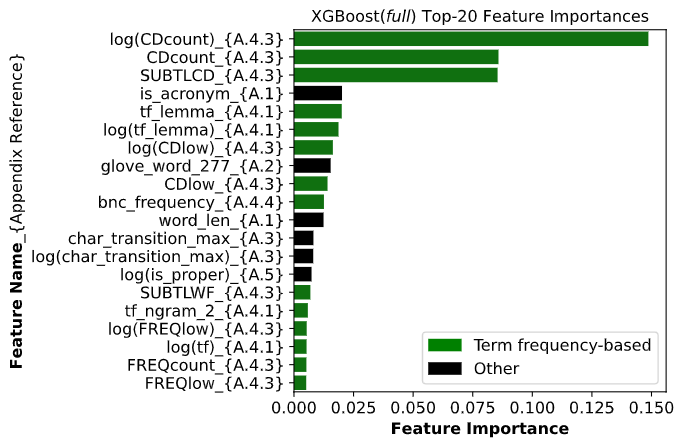
\includegraphics[scale=0.45]{xgboost_feature_importances.png}
  \captionsetup{justification=centering}
  \caption{\label{fig:xgboost_feature_importance} Feature importances for XGBoost(\textit{full}).}
\end{figure}

In total we consider 110 features, in addition to our multidimensional embedding-based features and $\log$-transformed features. We inspect the estimated feature importance scores produced by the XGBoost(\textit{full}) model to find that term frequency-based features (eg. unigrams, bigrams, trigrams) are of overwhelming importance (see Figure \ref{fig:xgboost_feature_importance}). This raises concern for whether the MT-DNN model too relies on term frequencies to make \textit{its} predictions, and if not, the linguistic features it may have learned upon fine-tuning. Of the remaining features having non-zero feature importances, most appear to be dimensions of a target word-based semantic feature (ie. GloVe or ELMo embeddings).

\subsection{BERT Attention}
\label{sec:bert_attention}

\begin{figure}
  \centering
  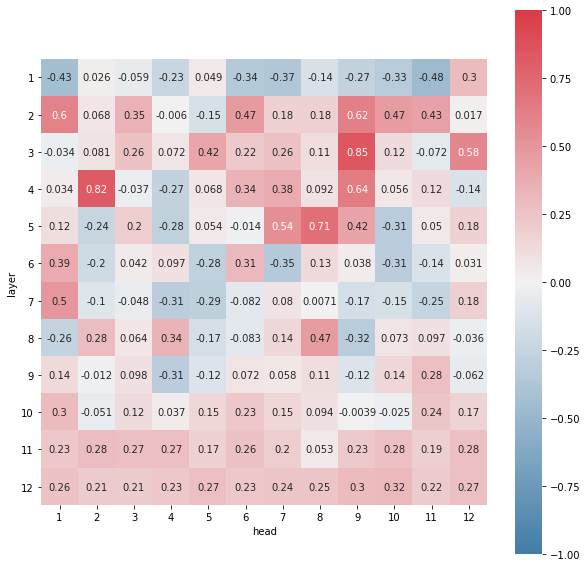
\includegraphics[scale=0.375]{head_correlations_tf.png}
  \captionsetup{justification=centering}
  \caption{\label{fig:head_correlations_tf} Attention head correlation between word frequency and total attention received by word, averaged across 100 random test set samples.}
\end{figure}

\begin{figure}
  \centering
  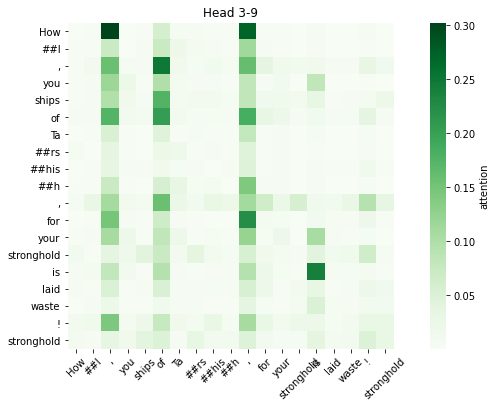
\includegraphics[scale=0.45]{head_3-9.png}
  \captionsetup{justification=centering}
  \caption{\label{fig:head_3-9} Head 3-9 attention map for a random sample.}
\end{figure}

Attention maps have in previous works been assessed to demonstrate linguistic phenomena learned by a Transformer's specialized attention heads \citep{190509418, 190604341}. We extract attention maps from MT-DNN's underlying fine-tuned BERT architecture. For each sample in the single word test set, we obtain an attention map from each of the BERT base model's 144 attention heads (ie. 12 heads per 12 layers).

Based on the precedence given to term frequency features by the XGBoost(\textit{full}) model, we hypothesize that for certain attention heads, the degree to which BPEs attend to one another varies relative to their word's rarity in lexicon. This follows the findings of \citet{190509418}, who identify heads in which lesser frequent tokens are attended to semi-uniformly by a majority of sentence tokens. 

To test our hypothesis, we estimate for each attention head the Pearson correlation between word frequency and average attention given to each word in the context.\footnote{We compute attention given to a \textit{word} as the sum of attention given to its constituent byte pair encodings (BPEs). We use the GBND corpus to extract word frequencies, though any large corpora would suffice.} As illustrated in Figure \ref{fig:head_correlations_tf}, we find multiple attention heads appearing to specialize at directing attention towards the most or least frequent words (depending on sign of the correlation). Vertical stripe patterns like that in Figure \ref{fig:head_3-9} emerge as a result of attention originating from a spectrum of tokens. The findings seem to affirm the fundamental relevancy of word frequency to lexical complexity prediction, corroborating our intuition.

\section{Conclusion}

In this paper, we report inspirations for systems submitted by \texttt{BigGreen} to LCP SharedTask 2021, achieving reasonable performance for the single word subtask by adapting ensemble methods upon feature engineering and feature learning-based models. We see potential in future deep learning approaches, acknowledging the need for complementary word frequency-based handcrafted features for the time being. We surpass our submitted results for the MWE subtask, by utilizing the predictive capabilities of our single word subtask models.

Avenues for improvement include better data aggregation, as the relative lack of class-4,5 samples hurts Pearson correlation across extremely complex samples. An approach may involve synthetic data generation using SMOGN \citep{pmlrv74branco17a}. \citet{shardlow2020complex} acknowledge a reader's familiarity with a genre may affect perceived word complexity. However, the CompLex dataset lacks information on each annotator's expertise or background, which may offer valuable new insights.

\bibliographystyle{acl_natbib}
\bibliography{anthology,acl2021}

%\appendix

\end{document}
